\setcounter{section}{1}
\section{Сумма на отрезке в статическом массиве: префиксные суммы.}

\textbf{Определение.} \textit{Префиксная сумма} по $j$ элементам - это сумма первых $j$ элементов массива.

\textbf{Основная задача.} Есть массив из $n$ элементов $a_1, \ldots, a_n$ и $q$ запросов вида $(l_1, r_i), ..., (l_q, r_q)$. Требуется для каждого запроса вывести $\sum\limits_{j = l_i}^{r_i}a_j = a_{l_i} + a_{l_i + 1} + ... + a_{r_i}$, где $i$ - номер запроса. 

\textit{Решение:} Посчитаем префексные суммы для любого $j$ от $0$ до $n$: $pref_j = a_1 + ... + a_j$. Для $j = 0: pref_0 = 0$, для $j > 0: pref_j = pref_{j-1} + a_j$. Ответ на запрос $(l_i, r_i):$ $\sum\limits_{j = l_i}^{r_i}a_j = pref_{r_i} - pref_{l_i - 1}$.

\textit{Ассимптотика:} Подсчёт всех значений $pref_j$ (по порядку) займёт $O(n)$ времени, подсчёт ответа на все запросы: $O(q)$. Итоговая ассимптотика $O(n + q)$. 

\textbf{Замечание.} В нашей модели вычислений считывать, складывать и умножать числа можно за $O(1)$.

\setcounter{section}{2}
\section{Проверка вхождения числа x в отсортированный массив: бинарный поиск.}

\textbf{Основная задача.} Проверить, есть ли заданный элемент $x$ в упорядоченном массиве $a_1, ..., a_n$. Если есть, вернуть
позицию его первого вхождения. Если нет, вернуть -1.

\textit{Решение: \textbf{(Бинпоиск)}} 
Шаг. Сравниваем элемент в середине массива (медиану) с заданным элементом $x$. Выбираем нужную половину массива в зависимости от результата сравнения. Повторяем этот шаг до тех пор, пока размер массива не уменьшится до 1.

\textit{Ассимптотика:} 
С каждым шагом размер массива уменьшается в $2$ раза. Следовательно, чтобы размер отрезка стал равен $1$, нужно $\log(n)$ шагов. Шаг занимает $O(1)$ времени. Итоговая ассимптотика $O(\log(n)).$ 

\textit{Реализация:}

\lstinputlisting[language=C++,
emph={int,char,double,float,unsigned},
emphstyle={\color{blue}}
]{code/2-5_binfind.cpp}

\setcounter{section}{3}
\section{Структура данных стек: реализация на указателях.}

\textbf{Стек (односвязный список)} - абстрактный тип данных, представляющий собой список элементов, поддерживающий следующие операции: 

1) Добавление числа в конец.

2) Вывод и удаление последнего числа.

\subsection*{Реализация на указателях}

Реализация стека на указателях - структура, в которой каждому элементу стека соотвествует ячейка, в которой хранится значение элемента и указатель на ячейчку предыдущего элемента. (в первой ячейке можно хранить указатель на nullptr).

При добавлении элемента создаётся новая ячейка, в которую записывается значение элемента, а также ссылка на конечную ячейку стека. Запоминаем, что теперь новая ячейка является конечной в стеке.

При удалении: запоминаем, что предпоследняя ячейка стека теперь является конечной. Удаляем ячейку, которая до этого была конечной.

\begin{figure}[h]
\begin{center}
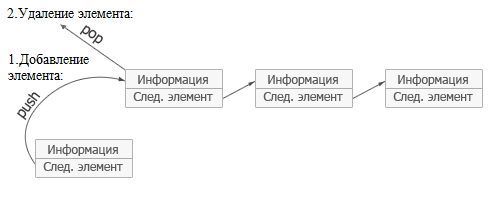
\includegraphics[width=0.7\linewidth]{images/2-5_stack_nodes}
\label{fig:mpr}
\end{center}
\end{figure}

\textit{Ассимптотика:} Все опрерации за $O(1)$.

\textit{Реализация:}

\lstinputlisting[language=C++,
emph={int,char,double,float,unsigned},
emphstyle={\color{blue}}
]{code/2-5_stack_node.cpp}

\setcounter{section}{4}
\section{Поиск ближайшего меньшего/большего слева/справа в статическом массиве.}

\textbf{Основная задача.} Дан статический массив $a_1, ..., a_n$. Определим $\forall i \in \{1, ..., n\} \ f(i) = max\{j < i \ | \ a_j > a_i\}$ (Для любого $i$ ищем ближайший слева элемент больший $a_i$).

\textit{Наивная реализация:} $O(n^2)$. Для каждого $i$ проходимся по всем $j < i$.

\textit{\textbf{Реализация с использованием стека:}}

При посчёте ответа для $i$ можно использовать данные, полученные при посчёте ответа для $i - 1$. В стеке будем хранитить значения, которые могут стать ответом. При $i = 1$ стек пуст. Ответ, очевидно, $f(1) = -1$ (т.е. нет ответа). Делее ищем $f(i)$ для всех $i$ по порядку. При $i = k$: Удаляем все элементы небольшие $a_k$ из стека. Такие элементы лежат только в конце стека. Они не могу являться ответом не только для $i = k$, но и для $i > k$, так как $a_k$ лучше будет подходить под ответ. Последний из элементов, оставшихся в стеке, будет ответом. (либо -1, если стек пуст) Далее в стек добавляем $a_k$. Можно заметить, что элементы в стеке лежат в порядке убывания по значению и в порядке возрастанию по индыксу, в данном нам массиве. 

\begin{figure}[h]
\begin{center}
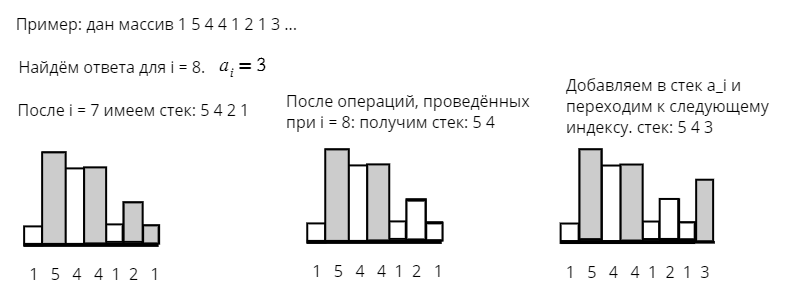
\includegraphics[width=0.9\linewidth]{images/2-5_stack_5_2}
\label{fig:mpr}
\end{center}
\end{figure}

\textit{Ассимптотика:} Так как каждый элемент был в стек ровно 1 раз, а потом мог быть удалён, то время работы алгоритма $O(n)$. 

\textit{Код:}

\lstinputlisting[language=C++,
emph={int,char,double,float,unsigned},
emphstyle={\color{blue}}
]{code/2-5_stack_5.cpp}

\textbf{Утверждение.} После выполнения $i$-ой итерации цикла for в стеке будут лежать числа:
$...,f(f(i)), f(i), i$.

$\blacktriangle$ На каждой итерации $j$ за значение $f(j)$ берётся последнее число в стеке, после чего в стек добавляется $j$. Следовательно, любые два подряд идущих элемента в стеке имею вид $f(q), q$. После выполнения $j$-ой итерации в стек всегда кладут $j$. Следовательно, после выполнения $i$-ой итерации цикла for в стеке будут лежать числа:
$...,f(f(i)), f(i), i. \quad \blacksquare$

\setcounter{section}{5}
\section{Поддержка минимума в стеке.}

Необходимо написать структуру (стек), которая поддерживает следующие операции:

1) push

2) pop

3) top

4) min - минимум среди элементов стека.  

\textit{Алгоритм:}
Используем стек на указателях, но в каждой ячейке будем хранить 3 значения $\{val, min, prev\}$: число, минимум среди элементов стека, лежащих под ним, ссылку на предыдущую ячеёку стека. 

1) \textit{push}. Добавляем число $x$ в стек. Переменной $min$, добавленной ячейки, присваиваем минимум из $x$ и значения $min$ из предыдущей ячейки.

2) \textit{pop}. Удаляем верхнее число (ячейку) из стека.

4) \textit{min}. Выводим значение $min$ из верхней ячейки.

\begin{figure}[h]
\begin{center}
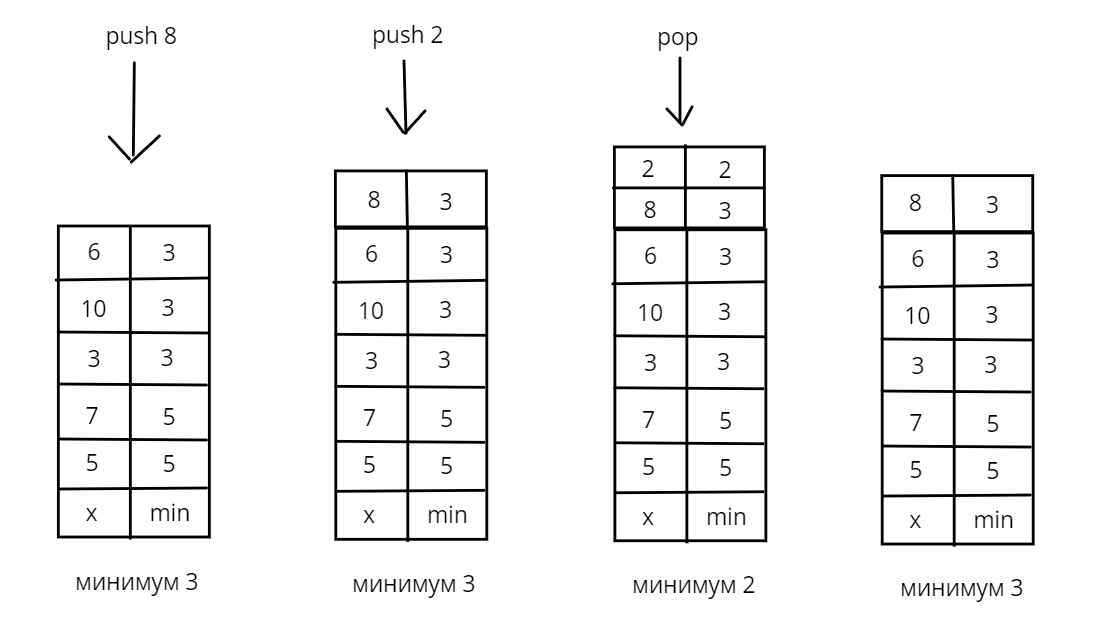
\includegraphics[width=0.9\linewidth]{images/2-5_stack_min}
\label{fig:mpr}
\end{center}
\end{figure}